\documentclass{report}

\usepackage{amsmath}
\usepackage{graphicx}
\usepackage{url}

\author{Martin Knudsen}
\title{Diagonalisation of random real symmetric matrices}


\begin{document}
\maketitle

\section*{Introduction}
I am solving problem $27$ in \cite{fedorov}. 
The problem is to implement a function that given an integer makes a $n x n$ random real symmetric matrix with elements chosen uniformly at random in the interval $[0, 1]$. The matrix then has to be diagonalized and in the proces finding the largest eigenvalue which is returned. This proces is repeated for different values of n, which results in data for a plot and a fit. 


\section*{Method}
I have solved this problem using $c$ and specifically the $gsl$ package. I have created a function that takes a number $n$ and creates a symmetric real matrix $M$ of size $n$ with random entrances usig $gsl\_matrix$ and the $rand()$ function from $stdlib.h$. I have then used the $gsl\_eigen\_symm$ function and workspace to find the eigenvalues of the matrix by diagonalizing it. Then the $gsl\_sort\_vector()$ function was used to find th the largest eigenvector, which was returned. This proces was repeated for $n=1, n=2\cdots n=100$. 
\begin{figure}[tbhp]
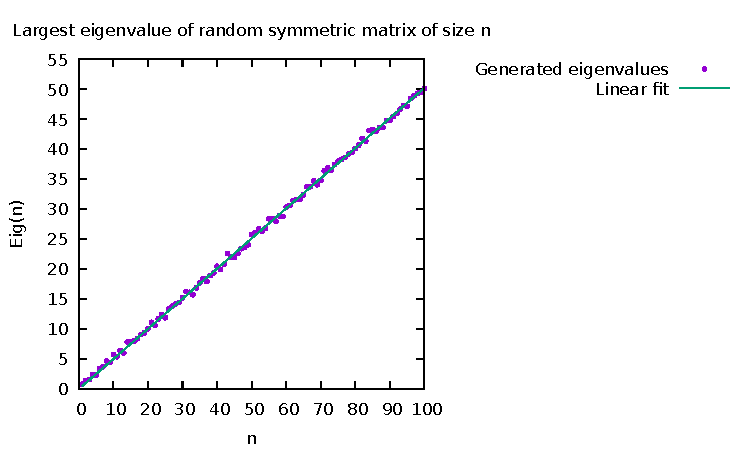
\includegraphics[width = \textwidth]{Eigenvalue}
\caption{The largest eigenvalue as a function of matrix size n for random symmetric real matrices. The purple dots represent the found eigenvalues while the green line represent a linear fit to the data using equation \eqref{eq:fit} \label{fig:eigen}}
\end{figure}

To fit the data I have used a simple linear fit without constant offset as in equation \eqref{eq:fit}. 
\begin{equation}
y = cx
\label{eq:fit}
\end{equation}
$gsl\_fit\_mul()$ was used to perform the fit. The value of the single fitting parameter as found by $gsl\_fit$ is $c=0.502276$ which is very close to being $0.5$ which we would expect since the entrances of the matrix are random numbers in the range $[0,1]$ which should converge to 0.5. The fit can be seen on figure \ref{fig:eigen}.  




% Bibliographystuff
\bgroup
\let\clearpage\relax
\begin{thebibliography}{9}

\bibitem{fedorov}
Fedorov, D.V., 
Retrieved 14.03.2018, 
from \url{http://86.52.112.181/~fedorov/prog/ass/sf.pdf}.

\end{thebibliography}
\egroup

\end{document}